%!TEX encoding = UTF-8 Unicode
\documentclass{lecturenotes}

\setbeamertemplate{footline}[frame number]
\title[Scala as a beginner language]{Scala as a Beginner Language}
\subtitle{-- Experiences and plans at LTH}
\author{Björn Regnell}
\institute{Datavetenskap, LTH}
\date{2016 April 20}

\begin{document}

\frame{\titlepage}
\frame{Agenda\tableofcontents}

%%% EXPERIENCES

\section[Experiences with Scala at LTH]{Experiences with Scala as a beginner language at LTH}

\subsection[Scala at LTH Science Center Vattenhallen]{Primary school activities at LTH Vattenhallen}

\begin{Slide}{Primary school activities at LTH Science Center Vattenhallen}
\begin{multicols}{2}

\footnotesize
\begin{itemize}
\item \Alert{Thousands of school kids} visiting Vattenhallen have done \Emph{programming experiements} using LTH's free teaching material in Scala and Kojo:
\href{http://www.lth.se/programmera/uppdrag}{www.lth.se/programmera/uppdrag} \\ \Alert{Try it yourself!}

\item \Alert{Hundreds of teachers} have taken LTH's \Emph{programming courses for primary school teachers} 

\item We are supporting \Emph{Skolverket} with coming curricula plans. \\\Alert{AT LAST:}\\ \Emph{Programming in school!!!}




\end{itemize}
\columnbreak
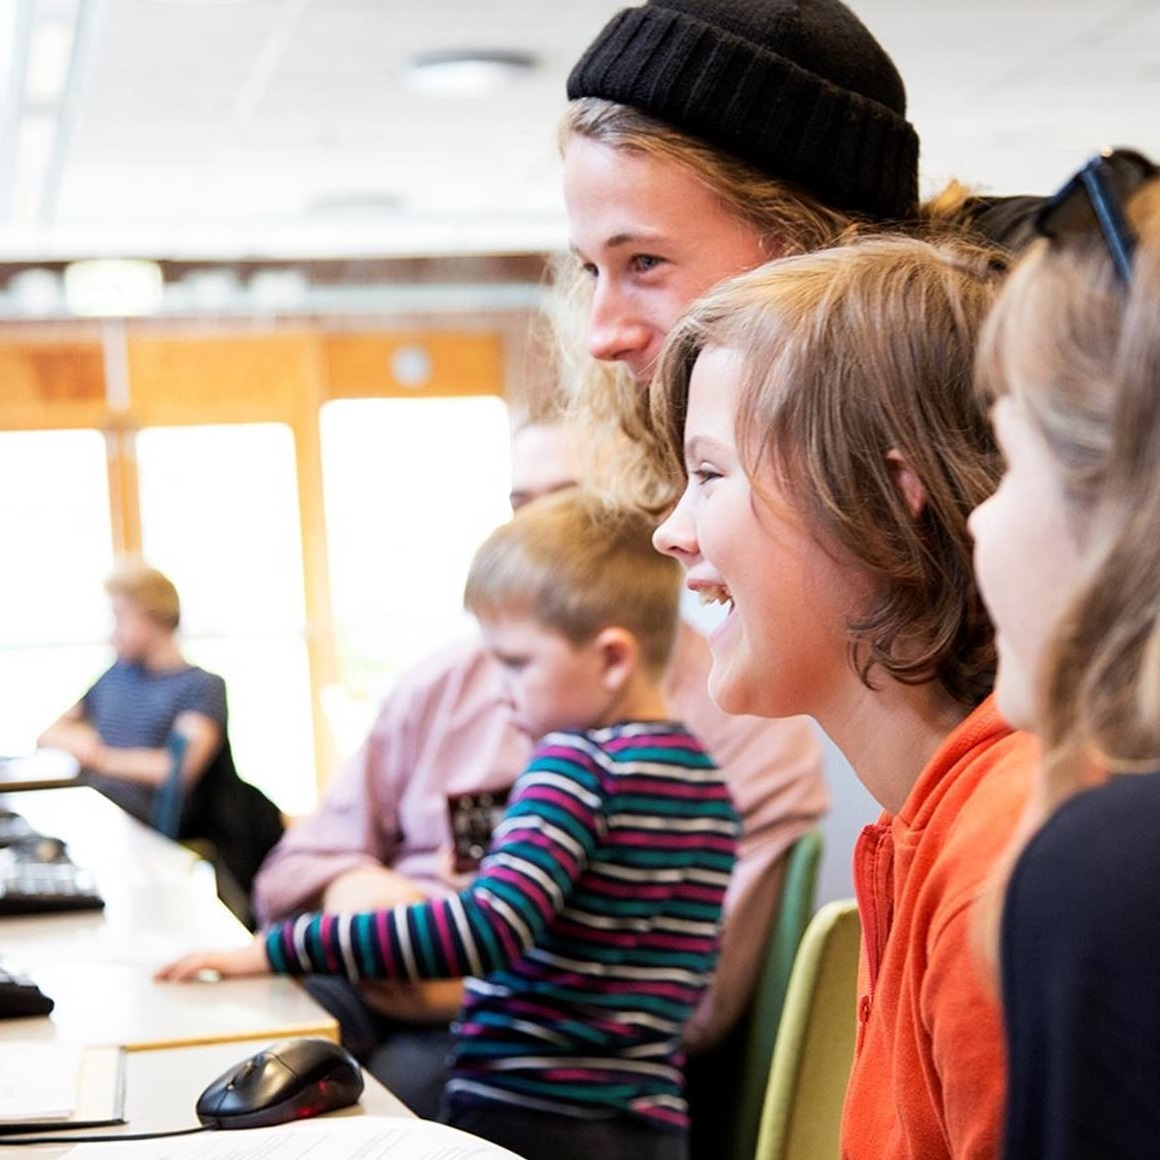
\includegraphics[width=0.6\textwidth]{../../img/kids}
\end{multicols}

\end{Slide}

\subsection[Turtle graphics in Scala with Kojo]{Turtle graphics in Scala with Kojo in Swedish}

\begin{Slide}{Scala for Kids: Programming unplugged}
\begin{multicols}{3}
\begin{itemize}
\item \Alert{S}equence
\item \Alert{A}lternative
\item \Alert{R}epetition
\item \Alert{A}bstraction
\end{itemize}
\columnbreak
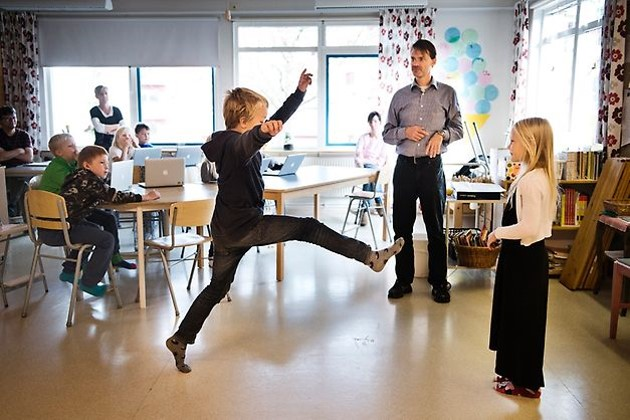
\includegraphics[width=0.7\textwidth]{../../img/unplugged}
\end{multicols}
\end{Slide}


\begin{Slide}{Scala for Kids: Turtle graphics in Kojo}
\begin{multicols}{2}
\begin{itemize}
\item \Alert{S}equence
\item \Alert{A}lternative
\item \Alert{R}epetition
\item \Alert{A}bstraction
\end{itemize}
\columnbreak


{
\includegraphics[width=0.5\textwidth]{../../img/kojo/stairs}}

\end{multicols}
\end{Slide}


%%% PLANS

\section[Plans for Scala at LTH]{Future plans for Scala as a beginner language at LTH}

\subsection[Potential pedagogical benefits and risks]{Potential pedagogical benefits and risks}


\subsection[New course: EDAA45 ''Introduction to programming'']{New course: EDAA45 ''Introduction to programming''}

\begin{Slide}{Student participation in teaching development through open sourcing of teaching material}

{\large\textbf{\url{https://github.com/lunduniversity/introprog}}}

\begin{multicols}{3}\footnotesize
Anders Buhl, \\Anna Palmqvist Sjövall, \\Anton Andersson, \\Casper Schreiter, \\Cecilia Lindskog, \\Christine Boghammar, \\Emil Wihlander, \\Emma Asklund, \\Erik Bjäreholt, \\Erik Grampp, \\Erik Söderbarg, \\Filip Stjernström, \\Fredrik Danebjer, \\Gustav Cedersjö, \\Henrik Olsson, \\Jacob Bohlin, \\Jakob Hök, \\Johan Ravnborg, \\Jonas Danebjer, \\Maj Stenmark, \\Maximilian Rundgren, \\Måns Magnusson, \\Oscar Sigurdsson, \\Oskar Berg, \\Oskar Widmark, \\Povel Larsson, \\Sebastian Hegardt, \\Stefan Jonsson, \\Tom Postema, \\Valthor Halldorsson, \\Viktor Claesson
\end{multicols}

\Emph{Contributions are welcome!}
\end{Slide}


\begin{Slide}{TITLE}
\begin{itemize}
\item SOME ITEM
\end{itemize}
\end{Slide}

\end{document}
